\documentclass[article,a4paper]{IEEEtran}
\usepackage[backend=biber]{biblatex}
\usepackage{graphicx}
\usepackage{lipsum}

\addbibresource{refs.bib}
\title{Powering the Future: Energy Harvesting and Intermittent Computing in IoT}
\author{
\IEEEauthorblockN{Anton Odén}\\
\IEEEauthorblockA{Dept. of Maths and Computer Science\\Karlstad University\\
651 88 KARLSTAD, Sweden}\\
anton.oden@outlook.com
}

\begin{document}

\maketitle

\begin{abstract}
    
\end{abstract}

\tableofcontents
\subsection{Introduction}
%\subsubsection{The need for sustainable computing}
%\subsubsection{How energy harvesting enables battery-free systems}
%\subsubsection{THe role of intermittent computing in IoT}

\subsection{Energy harvesting: A new power paradigm}
%\subsubsection{What is energy harvesting?}
Energy harvesting refers to the process of capturing and converting ambient energy from natural or artificial sources into usable electrical power. Common sources of harvested energy include solar radiation, thermal gradient, mechanical vibration, biochemical reactions and readio frequencys \cite{Energyharvest1}. Unlike traditional power supplies, energy harvesting systems enable autonomous operation in environments where wired connection or battery replacements are impractical. This technique is increasingly vital for IoT devices, embedded systems with batter-free computing where maintaining continious power supply is challenging or that cutting the cost of battery is the next step in making IoT devices even more cheap.
\newline\newline 
%\subsubsection{RF energy harvesting and the WISP project}
One promising and intriging technology in energy harvesting is RF (radio frequency) energy harvesting, which ulitlizes electomagnetic waves from sources such as cell towers, WiFi signals and RFID readers to generate power. The WISP (Wireless indentification and sensing platform) project exemplifies this approach, demonstrating how RF energy can support battery-free computation and sensing. WISP operates using passive RFID technology, converting radio waves into energy enought for tasks like data processing and sensor driven applications. This enables devices to function in environments with consistens RF energy exposure, pawing the way for battery-free IoT solutions.
\newline 
%\subsubsection{Challenges in energy-harvesting}
Despite advantages of IoT devices able to compute and communicate without traditional battery. Energy harvesting does has a challenge with ambient energy fluctuation leading to unpredicable power levels. This leads to systems requeired to adopt intermittent computing strategies such as e.g. Alpaca, Ratchet and Chinchilla further discussed in this article. 
\begin{figure}
    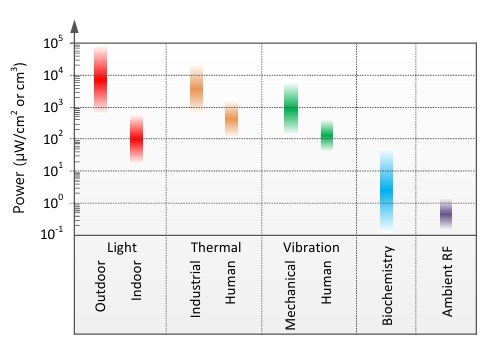
\includegraphics[width=\columnwidth]{EnergyHarvest1.png}
    \caption{ Different energy harvesting areas showing given energy from \cite{Energyharvest1} }
    \label{fig1_Energy_harvest }
\end{figure}

\subsection{Understanding intermittent computing}
Intermittent computing is designed for systems that experience frequent power interruptions, often seen in energy-havesting devices. Unlike traditional computing, which assumes continious power availability, intermittent systems must exccute tasks in small steps, ensuring progress even during power failures. 
%\subsubsection{Why traditional computing fails under unstable power?}
Counter to traditional computing that could be considered to be continious. Intermitted computing is able to handle planned or unplanned breaks in computation. The processor in itself does not have a problem with powerbreaks but the memory used in computation to write and read data is more or less stored in volatile memory, for example RAM, Cache, CPU registers. Meaning that it doesn't uphold data during power loss. Memory that does keep data during powerloss is non volative and could be for example FRAM, Flash, EEPROM. Traditional computing then fails under unstable power as memory used by computation is lost and there is no checkpoints to know what state the computation and memory was in close to power loss so the computation results can't be trusted to be correct if it wouldn't restard from beginning. Energy harvesting dependent systems has to operate intermittent as the energy harvested can't assumed to be constant, but instead is loosing power frequently and unexpectedly. 
%\subsubsection{Strategies for reliable compution with energy harvesting}
Since power availability differs in energy-harvesting systems, computing strategies must adapt. Some key approaches include, \textbf{checkpointing} that regularly saves system state so computation can resume at last checkpoint (e.g. Chinchilla and Ratchet). \textbf{Task-based execution} where program is broken into small self-contained taskes that restarts after power loss (Alpaca). \textbf{Non-volatile memory} usage, storing of exceution data in FRAM or Flash memory to preserve progress. \textbf{Energy aware scheduling} that could dynamically adjust workload based on realtime power levbels, enruing tasks execute only when sufficient energy is available. 

\subsection{Frameworks for intermittent computing}
Intermittent computing requires specialized compilation techniques to ensure programs can funtion despite unpredicable power failures. Unlike traditional compilation, which assumes continuous execution, intermitent computing frameworks modify code execution behavior so systems can resume operations seamlessly after a power outage. These frameworks aim to prevent data loss when power fails, enable efficient recovery without manual intervention and optimize execution for low-power environments. 
\subsubsection{Why compilation matters for intermittent systems}
Since energu-harvetsing devices operate with instable power, normal software execution fails because variables, loop states and memory data disappear when power is lost. Specialized compilation frameworks enhance program by automatically adding checkpoints to preserve state (Ratchet) or adjusts checkpoint frequency dynamically based on power availability (Chinchilla). Also iterated computation statements could in compilation be flages as non-idempotent and temporary variables is added by compilers (Alpaca). 
\subsubsection{Ratchet: Automatic checkpointing without hardware support}
Ratchet provides compiler-based automatic checkpointing which makes it possible to use without hardware support, meaning standard microcontrollers could be used. Ratchet inserts checkpoints in compilation without requiring programmer to modify code manually. The checkpoints creates idempotent sections of the code where write and read (WAR)-instructions are separated to avoid problem that could arrise when program gets interrupted in the middle of a section. This is illusrated in \ref{fig2_WAR_problem} showing memory written affects computation on restart. 
\newline\newline
Ratchet transform execution state into safe recoverable snapchots, ensuring program resume smoothly after power loss. It enures redundancy is minimized to prevent unnecessary recomputation. THe code for Ratchet is open sourced since 2016 via \cite{Ratchetsrc}.
\begin{figure}
    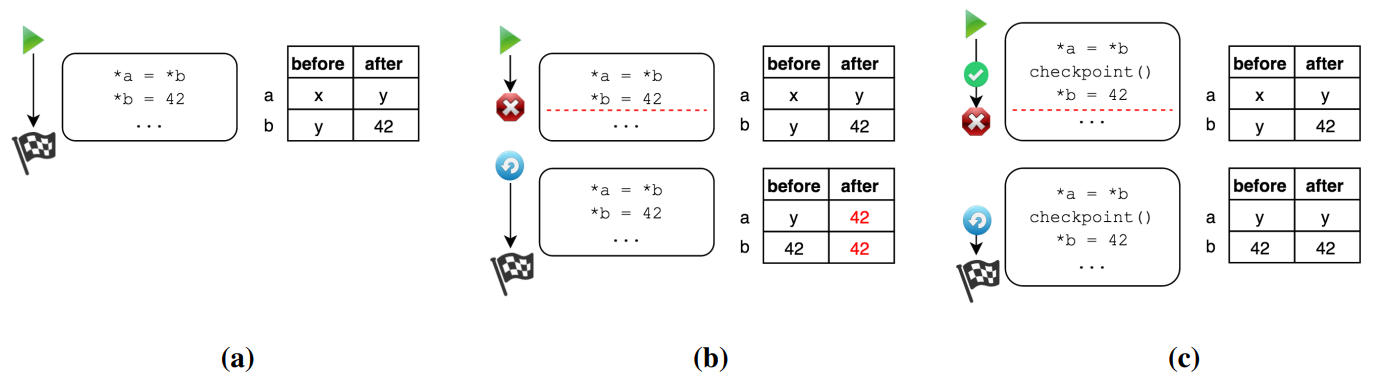
\includegraphics[width=\columnwidth]{WAR-problem.png}
    \caption{ Basic example illustrating difficulties with using non-volatile main memory on intermittent powered computers from \cite{Ratchet} }
    \label{fig2_WAR_problem}
\end{figure}
\subsubsection{Chinchilla: adaptive checkpoints for efficient computing}
Chinchilla introduces dynamic checkpointing that adjust checkpoint frequency based on avail energy to maximize efficiency. This ensures minimal overhead by choosing only necessary checkpoints instead of static as in Ratchet. 
\subsubsection{Alpaca: Task-based programs for software resilience}
In Alpaca more work is on the programmer to divide programs into shunks of tasks. The programmer needs to be aware of the amount of energy that is possible at a minimum to compute with so a task is not to large and thereby not able to finish. As the program overhead is handed to the programmer there is more room for designing efficient code adapted to the device environment which could differs largeely between devices. Overhead is limited to every individual task write to non volatile memory at the end of a task. Second feature-leg for Alpaca is privatization that guarantees that volatile or non-volatile memory access by a task remains consistent, regardless of power failure. 
\newline\newline
Alpaca divides data into task-shared and task-local data. Task-shared variables are in the global scope and are allocated in non-volatile memory and once a task writes a value to a task-shared variable, that same task or another task may later read the value. In Alpaca the compiler backtracks write and reads to all task-shared variables to decide if tasks needs to privatize usage of variables, meaning that a local variable is created in tasks and in the end of task a commit to task-shared variable is done before transitioning to next task. Task-local variables are scoped only to a single task and must be initialized by that task and are allocated in volatile memory.
\newline\newline
Committing of data from volatile to non-volatile memory is done in two phases and flags are changed to signal what phase the task was in when rebooting after power interruption. First pre-commit creates a table in non volatile memory with all values to be changed in the task-shared scope. If interrupted during this phase the whole task needs to be computed from beginning. After pre-commits done, commit\_ready is set to \texttt{true} and Alpaca runtime during reboot knows to jump to commitphase directly. In commit phase task-shared variables are changed in non-volatile memory. When commitphase is done commit\_ready flag i removed and end-index is set to zero. So that the Alpaca runtime knows that transition to next task is the only step left to do on reboot. To support privatization the programmer needs to specify task-shared variables for Alpaca to guarantee consistency of data.
\newline\newline
Alpaca was developed by Kian Maeng, Alexei Colin and Brandon Lucia at Carnegie Mellon University in USA with presentation of its work 2017. The sourcecode for runtime enironment can be found on github \cite{Alpacasrc}. It has been developed in differerent versions as the text in \cite{Alpaca} presents Alpaca-redo, Alpaca-undo and Alpaca-VM that uses the same approach of dividing program into taskes but handles the memory in different fashion. The privatization of data and commitphases prior described follows the Alpaca-redo runtime system. Alpaca-undo does instead work with variables in task-shared scope directly but does keep a list och back-up variables that writes over changes done to task-shared variables in case of power failure. This makes Alpaca-undo more efficient than Alpaca-redo for systems that are assumed to not have a task powerfail more often than succeding computation.  
\begin{figure}
    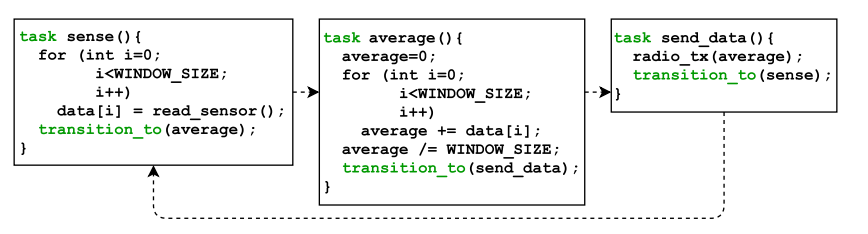
\includegraphics[width=\columnwidth]{Alpacatasksexample.png}
    \caption{ Example application written i Alpaca from \cite{Alpaca} }
    \label{fig3_Alpaca_tasks}
\end{figure} 

\subsection{Future directions and applicaitons}
Hello Hellol Hello
%\subsubsection{Expanding energy harvesting in IoT}
%\subsubsection{Optimizing frameworks for Low-Power Devices}
%\subsubsection{Open challenges and research opportunities}

\subsection{Conclusion}
%\subsubsection{Key takeawats from Energy harvesting and intermittent computing}
%\subsubsection{THe path towards sustainable, battery-free computing}
In this article we have discussed intermittent computing, energy harvesting of radio waves and how IoT could potential power much itself by sheer device volume.

Intermittent computing adds a layer of consideration for the programmer and designer of device. We have highighted Ratchet, Chinchilla and Alpaca that are three approached to tacle the problem of keeping track of programstate with power interruptions that devices being reliate on energy harvesting only has. But of cource power interruptions could happen otherwise also so the concepts of adding checkpoints is applicable in a broader sence altought this article focuses on smaller IoT devices. 
\printbibliography

\end{document}